% This is part of Un soupçon de mathématique sans être agressif pour autant
% Copyright (c) 2015
%   Laurent Claessens
% See the file fdl-1.3.txt for copying conditions.

\begin{exercice}[\cite{NRHooXFvgpp5}]\label{exo2smath-0126}

Déterminer, dans chaque cas, l'échelle utilisée.
\begin{enumerate}
    \item
 Sur une carte routière, la distance entre deux villes est de \SI{15}{\centi\meter}. En réalité, cette distance est de \SI{300}{\kilo\meter}.
\item
    Sur la maquette d’un building, la flèche de l'immeuble mesure \SI{12}{\centi\meter}. En réalité, elle mesure \SI{36}{\meter}.
\item
    Une Tour Eiffel en modèle réduit mesure \SI{18}{\centi\meter}. En réalité, elle mesure \SI{324}{\meter} (antennes de télévision incluses).
\item
    Ceci est la photo d'un pou\cite{OUDMooPWBllL} :
    \begin{center}
 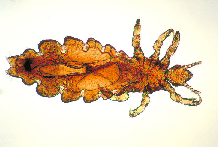
\includegraphics[width=5cm]{Pediculus_humanus.pdf}
    \end{center}

\end{enumerate}

\corrref{2smath-0126}
\end{exercice}
